\subsection{Extrema d'une fonction a plusieurs variable}

\lecture{18}{2025-04-16}{Cours}{}

\begin{parag}{Point historique}
    oui
\end{parag}
\begin{parag}{Rappel}
    Soit un ensemble ouvert $E \subset \mathbb{R}^n$ contenant un point $a \in E$ et $f : E \to \mathbb{R}$de classe $C^3\left(E\right)$.\\
    Alors $f$ s'écrit:
    \begin{equation} f\left(x\right) = P_2f_a\left(x\right) + \epsilon\left( \mid \mid x - a \mid \mid^2\right) \end{equation}
    Avec le polynôme de taylor de $f$ d'ordre $2$: autour de $\left(a, b\right)$ tel que:
    \begin{equation} P_2f_a\left(x\right) = f\left(a\right) + < \nabla f\left(a\right), x - a> + \frac{1}{2}\left(x-a\right)^T \text{Hess}f\left(a\right)\left(x-a\right) \end{equation}
\end{parag}
\begin{parag}{Extrema d'une fonction de plusieurs variable}
    \begin{definition}
    Soit $E \subset \mathbb{R}^n$ et $f: E \to \mathbb{R}$ alors on appelle $a \in E$ un \important{point stationnaire} si $\nabla f\left(a\right) = 0$
    \end{definition}
    
\end{parag}
\begin{parag}{Extremum local}
    \begin{definition}
    La fonction $f: E \to \mathbb{R}$ admet un \important{maximum local (resp. minimum local)} au point $a \in E $ s'il existe $\delta > 0$ tel que pour tout $x \in E \cap B\left(a, \delta\right)$ on a $f\left(x\right) \leq f\left(a\right)$ (resp. $f\left(x\right) \geq f\left(a\right)$
    \end{definition}
    \begin{subparag}{Proposition}
        si $a \in E$ est un extremum local et $\nabla f \left(a\right)$ existe, alors $a$ est un point stationnaire $\left(\nabla f\left(a\right) = 0\right)$
        
    \end{subparag}
    \begin{subparag}{Proposition}
        Soit $g_i\left(x\right) = f\left(a_1, \ldots, a_{i-1}, x, a_{i+1}, \ldots, a_n\right)$.\\
        Par nos hypothèses, $g_i'\left(a_i\right)$ existe et $g_i\left(x\right)$ admet un extremum local en $x = a$ et donc, $g_i'\left(a_i\right) = 0$. Vu que $\frac{\partial f}{\partial x_i}\left(a\right) = g_i'\left(a_i\right) = 0$, et que l'argument s'applique pour tout $i = 1, \ldots, n$, on a  $\nabla f\left(a\right) = 0$.
    \end{subparag}
    \begin{subparag}{Remarque}
        La réciproque est fausse, $\nabla f\left(a\right) = 0$ n'implique par que $a$ est un extremum local.
    \end{subparag}
\end{parag}

\begin{parag}{Selle}
    \begin{definition}
    Un point stationnaire qui n'est pas un extremum local est un \important{point selle} de $f$.
    \end{definition}
    
    \begin{subparag}{Exemple}
        Si $f\left(x, y\right) = x^2 - y^2$, alors $\nabla f\left(x, y\right) = \left(2x, -2y\right)$ s'annule au point $\left(0, 0\right)$, mais ce n'est pas un extremum local.
    \end{subparag}
\end{parag}
        
       \begin{parag}{Point critique}
           \begin{definition}
            $a \in E$ est un point critique de $f : E \to \mathbb{R}$ si $a$ est un point stationnaire $\left( \nabla f\left(a\right) = 0\right)$, ou bien au moins une dérivées partielles de $f$ n'existe pas en $x = a$.
           \end{definition}
           \begin{theoreme}
           soit $f: E \to \mathbb{R}^2$ de classe $C^2\left(E\right), a \in E$ un point stationnaire, et $\lambda_i$ les valeurs propres de Hess de $f\left(a\right)$.
           \begin{itemize}
               \item $\forall i, \lambda_i > 0 \implies a$ est un minimum local
               \item $\forall i , \lambda_i < 0 \implies a$ est un maximum local
               \item $\exists i , j$ tels que $\lambda_i > 0$ et $\lambda_j < 0 \implies a$ est un point selle:
               
           \end{itemize}
           
           \end{theoreme}
           
       \end{parag}
       

       \begin{parag}{Résultat du théorème}
           Ce que nous dit ce théorème et que les Hessiennes peuvent nous dire si un point est un extremum local.\\
           Prenons comme exemple:
           \begin{equation*} f\left(x, y\right) = x^2 + y^2 \end{equation*}
           On a pour la Hessienne
           \begin{equation*} \text{Hess} f\left(0\right) = \begin{pmatrix} 2 & 0 \\ 0 & 2 \end{pmatrix} \end{equation*}
           On peut aussi prendre la fonction
           \begin{equation*} f\left(x, y\right) = x^2 - y^2 \end{equation*}
           On a pour la Hessienne:
                    \begin{equation*} \text{Hess} f\left(0\right) = \begin{pmatrix} 2 & 0 \\ 0 & -2 \end{pmatrix} \end{equation*}
   

                    Soit maintenant un dernier exemple:
                    \begin{equation*} f\left(x, y\right) = x^2 \end{equation*}
                    On a pour notre matrice:
         \begin{equation*} \text{Hess} f\left(0\right) = \begin{pmatrix} 2 & 0 \\ 0 & 0 \end{pmatrix} \end{equation*}
   
         Ce genre d'exemple sont pas très pratique car le théorème nous permet pas de faire le calcul a notre place.
       \end{parag}
       \begin{parag}{Esquisse de démonstration}
           La démonstration n'est pas parfaite, il y a des imprécisions.\\
           Si la fonction est de classe $C^2$, par le théorème de schwartz, on a que la Hessienne de $f\left(a\right)$ est symmetrique, alors cela implique que la Hessienne est diagonalisable.\\
           On écrit $\text{Hess}f\left(a\right) = ODO^T$ avec $O$ orthogonale et $D = \text{diag}\left(\lambda_1, \ldots, \lambda_n\right)$.\\
           De manière équivalente, on a Hess $f \circ O^T\left(a\right) = D$, un changement de variable $y = O^Tx$. \\
           On veut donc analyser notre fonction grâce au valeur propre de la Hessienne\\
           Par la formule de Taylor de $f\left(y\right)$ dans un voisinnage de $a$, on peut écrire de manière approciamtive:
           \begin{equation*} f\left(y\right) = f\left(a\right) + <\nabla f\left(a\right), y-a> + \frac{1}{2}\sum_{i = 1}^{n} \frac{\partial^2 f}{\partial y_i^2}\left(a\right)\left(y_i - a_i\right) + \epsilon\left( \mid\mid y - a\mid\mid^2\right)  \end{equation*}
           Ce qui si on l'approxime:
           \begin{equation*} \approx f\left(a\right) +   \frac{1}{2}\sum_{i = 1}^{n} \lambda_i\left(y_i - a_i\right)^2 \end{equation*}
           Ici on remplace la fonction directment par les valeurs propre de la Hessienne.
           Donc si $\lambda_i > 0$ on  a $f\left(y\right) \geq f\left(a\right)$, $\forall y$ dans un voisinage de $a \implies a$ est un minimum local de $f$. La ``faute'' ici est que l'on est entrain d'étudier le changement de variable de $f$ et non $f$ directement.

\begin{framedremark}
    Ici on a deux chose a ne pas confondre, $f \circ O^T\left(a\right)$ et $ODO^T$ qui n'ont pas le même produit, le premier ici prends un produit de matrice classique tandis que $f \circ O^T$ est une composition de fonction entre des fonctions dans $\mathbb{R}^n \to \mathbb{R}^p$.
\end{framedremark}
           
       \end{parag}
\begin{parag}{Remarque}
    Soit $c\left(t\right) = a + tv$ pour $v \in \mathbb{R}^n$. si $h\left(t\right) = f\left(c\left(t\right)\right)$ admet un minimum au point $0$ cela n'implique pas que $a$ est un minimum local de $f$.\\
    Si on prends la fonction $f\left(x, y\right) = \left(y-x^2\right)\left(y-2x^2\right)$ autour de $a = 0$, selon la droite $c\left(t\right) = t\left(u, v\right)$.\\
    On remplace par $c\left(t\right) = t\left(u, v\right)$:
    \begin{equation*} h\left(t\right) = \left(tv . \left(tu\right)^2\right)\left(tv - 2\left(tu\right)^2\right) = t^2\left(v^2 + q\left(t\right)\right) \end{equation*}
    \begin{equation*} h'\left(t\right) = 2t\left(v^2 + q\left(t\right)\right) + t^2q'\left(t\right) \end{equation*}
    Donc on redérive une fois encore pour pouvoir trouve les maximum est minimum locaux.
    \begin{equation*} h''\left(t\right) = 2v^2 + q\left(t\right) + 2\telque'\left(t\right) + t^2 q''\left(t\right) \end{equation*}
    On a que $h'\left(0\right) = 0$ et $h''\left(0\right) \geq 0$ et donc $0$ est un minium local de $h$.\\
    Cependant si on prends la courbe, $c'\left(t\right) = \left(t, \frac{3}{2}t^2\right)$ quand $t \neq 0$ on a des points proches de $\left(0, 0\right)$, mais tels que:
    \begin{equation*} f\left(c'\left(t\right)\right) = \left(\frac{3}{2}t^2 - t^2\right)\left(\frac{3}{2}t^2 - 2t^2\right) = -\frac{1}{4}t^4 < f\left(0, 0\right) \end{equation*}
    
    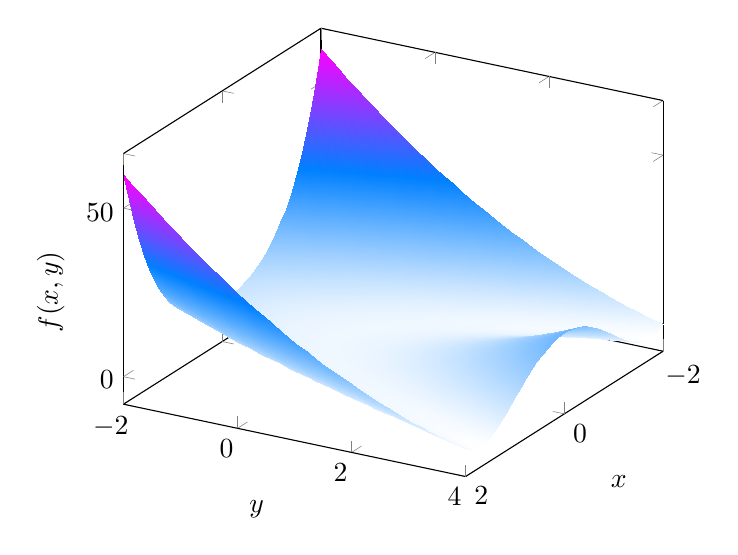
\begin{tikzpicture}
        \begin{axis}[
                view={120}{30},
                  xlabel={$x$},
                     ylabel={$y$},
            zlabel={$f(x,y)$},
                                domain=-2:2,
                                    y domain=-2:4,
                                        samples=40,
                                            samples y=40,
                                                colormap/cool,
                          ]
                \addplot3[
                        surf,
                        shader=interp,
                         ]
                         {(y - x^2)*(y - 2*x^2)};
         \end{axis}
         \end{tikzpicture}
    
\end{parag}

\begin{parag}{Théorème à connaître (condition équivalents sur Hess $f\left(a\right)$, cas $n = 2$}
    \begin{theoreme}
    La proposition suivante s'applique à tous les matrice symmétrique, donc on notre $H := \text{Hess} f\left(a\right) = \begin{pmatrix}r & s \\ s & t \end{pmatrix}$
    \begin{itzemize}
    \item $\lambda_1 > 0, \lambda_2 > 0 \iff \det H > 0$ et $r > 0$
    \item $\lambda_1 <0 , \lambda_2 < 0 \iff  \det H > 0$ et $r < 0$
    \item sgn $\left(\lambda_1\right) \neq $ sgn $\left(\lambda_2\right) \neq 0 \iff \det H < 0$
    \end{itzemize}
    
    \end{theoreme}
    
\end{parag}
\begin{parag}{Démonstration}
    Le déterminant et la trice de $H$ sont invariants par conjugaison. La diagonalisation $H = ODO^T$ donne alors:
    \begin{equation*} rt - s^2 = \det H = \det D = \lambda_1 \lambda_2 \end{equation*}
    \begin{equation*} r + t = Tr\,H = Tr\,D = \lambda_1 + \lambda_2 \end{equation*}
    \begin{subparag}{1 $\implies$}
        Supposons que $\lambda_1 > 0, \lambda_2 > 0$ immédiatement, on a que $\det H = \lambda_1\lambda_2 > 0$.\\
        Ensuite, $\lambda_1\lambda_2 = rt - s^2 > 0$ dont $rt > s^2 \geq 0 \implies$ $r$ et $t$ qui sont de même signe.\\
        De plus, $Tr\,H = \lambda_1 + \lambda_2 = r + t > 0$. On conclut que $r$ doit être strictement positif. (si la multiplication est positive \important{et} l'addition est positif).
    \end{subparag}
    \begin{subparag}{Dans l'autre sens}
        Suppsons que $\det H > 0$ et $r > 0$.\\
        Alors $\det H = \lambda_1\lambda_2 > 0 \implies \lambda_1$ et $\lambda_2$ sont de même signe.\\
        Ensuite, $\lambda_1 \lambda_2 = rt - s^2 > 0$ dont $rt > s^2 \geq 0$ mais $r > 0$ dont $t > 0$ aussi, $Tr\, H \implies r + t = \lambda_1 + \lambda_2 > 0$ et donc on utilise le même arguement que précédemment, $\lambda_1 > 0$ et $\lambda_2 > 0$.
    \end{subparag}
    \begin{subparag}{2}
        Le point 2 est laissé en exercice
        
    \end{subparag}
    \begin{subparag}{3}
        $\det H < 0 \iff \lambda_1\lambda_2 < 0 \iff \lambda_1$ et $\lambda_2$sont de signe opposés.
    \end{subparag}
    
\end{parag}

\begin{parag}{Critère de Sylvester}
    \begin{theoreme}
    Condition équivalentes aux condition suffisantes dans le cas $n = 3$.\\
    Soit $f \in C^2\left(E\right)$ au voisiange de $a$ tel que $\nabla f\left(a\right) = 0$.:\\
    Soit 
    \begin{itemize}
        \item $\Delta_1 = \det Hess_x f\left(a\right)$
        \item $\Delta_2 = \det Hess_{x, y}f\left(a\right)$
        \item $\Delta_3 = \det Hess_{x, y, z} f\left(a\right)$
        
    \end{itemize}
    Alors:
    \begin{itemize}
        \item $\Delta_1 > 0, \Delta_2, \Delta_3 > 0 \iff \lambda_1 > 0, \lambda_2 > 0, \lambda_3 > 0 \iff a$  est un minium local de $f$
        \item $\Delta_1 <0, \Delta_2 < 0 \delta_3 < 0 \iff \lambda_1 < 0 , \lambda_2 <0, \lambda_3 < 0 \iff a$ est un maximum local de $f$
           \item Autrement $\Delta_3 \neq 0 \implies \exists \lambda_i > 0$ et $\lambda_j > 0$ et $\lambda_j < 0 \implies a$ est un point selle de $f$
    \end{itemize}
    \end{theoreme}
\end{parag}
\begin{parag}{Exercice}
    Le  but est de trouver les points critique et de déterminer leur nature.\\
    Soit $f\left(x, y\right) = y^3 + 3y^2 - 4xy + x^2$. Alors $f \in C^{\infty}\left(\mathbb{R}^2\right)$ donc tout les points critiques trouvés sont stationnaire.\\
    On calcule
    \begin{equation*}  
 \nabla   f\left(x, y\right) = \left(-4y + 2x, 3y^2 + 6y - 4x\right) \end{equation*}
    Et Pour la Hessienne:
    \begin{equation*} \text{Hess} f\left(x, y\right) = \begin{pmatrix} 2 & -4 \\ -4 & 6y + 6 \end{pmatrix} \end{equation*}
    \begin{equation*} \nabla f\left(x, y\right) = 0 \iff \begin{cases} 2x = 4y \\ 3y^2 + 6y = 4x \end{cases} \iff \begin{cases} x = 2y \\ y\left(3y - 2\right) = 0\end{cases} \end{equation*} 
    Donc si on remplace ce qu'on trouve dans la Hessienne:\\
    On étudie donc les points stationnaire $\left(x, y\right) \in \{\left(0, 0\right), \left( \frac{4}{3},\frac{2}{3}\right)\}$
    Si on cherche donc les points selles:
    \begin{equation*} \text{Hess} f\left(0, 0\right) = \begin{pmatrix}2 & -4 \\ -4 & 6\end{pmatrix} \implies \det = -4 < 0 \end{equation*}
    Ce qui implique que le point $\left(0, 0\right)$ est un point selle.\\
    Si on prends donc Hess $f\left(\frac{4}{3}, \frac{2}{3}\right) = \begin{pmatrix} 2 & -4 \\ -4 & 10\end{pmatrix} = 4 > 0 \implies$ que ce point est un minimum local.
   

\end{parag}



       
       



